\chapter{MONTE CARLO CORRECTIONS AND SYSTEMATIC UNCERTAINTIES}
\label{chap:systematics}
Although great care has gone into the production of the simulated datasets used in this analysis, there are imperfections that lead to inaccuracies when compared to the data.
Running conditions were forced to change as the luminosity increased throughout the 2011 data taking, these changes lead to the largest discrepancies when comparing simulation to the data.
In order to account for the bias induced by the simulation inaccuracy, several corrections are performed to correct the simulation for comparison to the data.
In the process of correcting the simulation and due to other procedures there are a number of systematic and statistical uncertainties that need to be taken into account.
This chapter will discuss the corrections made to the simulation and the systematic uncertainties associated with the analysis.

\section{Monte Carlo Corrections}
\label{sec:montecarlocorrections}
The largest corrections to the Monte Carlo arise from inaccurate simulation of lepton selection and trigger efficiencies.
These efficiencies are measured in both the data and simulation, the simulation is then corrected to match the efficiency in the data whenever comparisons are made.
The efficiencies are measured through the use of the Tag \& Probe methodology\cite{TAGANDPROBE}.
In addition to corrections associated with the efficiency of selecting leptons, an additional event scale factor must be applied to account for differences in the pile-up interaction multiplicity between simulation and the data.

\subsection{Trigger Corrections}
\label{subsec:triggercorrections}
The trigger efficiency for the muon leg of a given trigger is measured by first assigning a tag muon that passes the isolated single muon trigger. 
Both the tag and probe muons are required to pass the full identification and isolation requirements outlined in Section \ref{sec:muonselection}.
Finally selected tag and probe muon pairs are only considered if the invariant mass of the di-muon pair lies within a window around the $Z$ mass ($60 < m_{\mu\mu} < 120$ GeV) and the muons have opposite sign.
An efficiency is measured as a function of $p_{T}$ of the probe muon by matching the probe muon to an isolated single muon trigger object.
A functional form of the trigger efficiency is determined by fitting an error function to the measured trigger efficiencies binned in $p_{T}$.
The derived functional form is the ``trigger turn on curve'' shown in the left hand portion of Figure \ref{fig:turnoncurve} with the barrel region on the top and the endcap region on the bottom.
\begin{figure}[ht]
\centering
\begin{minipage}[b]{0.45\linewidth}
\centering
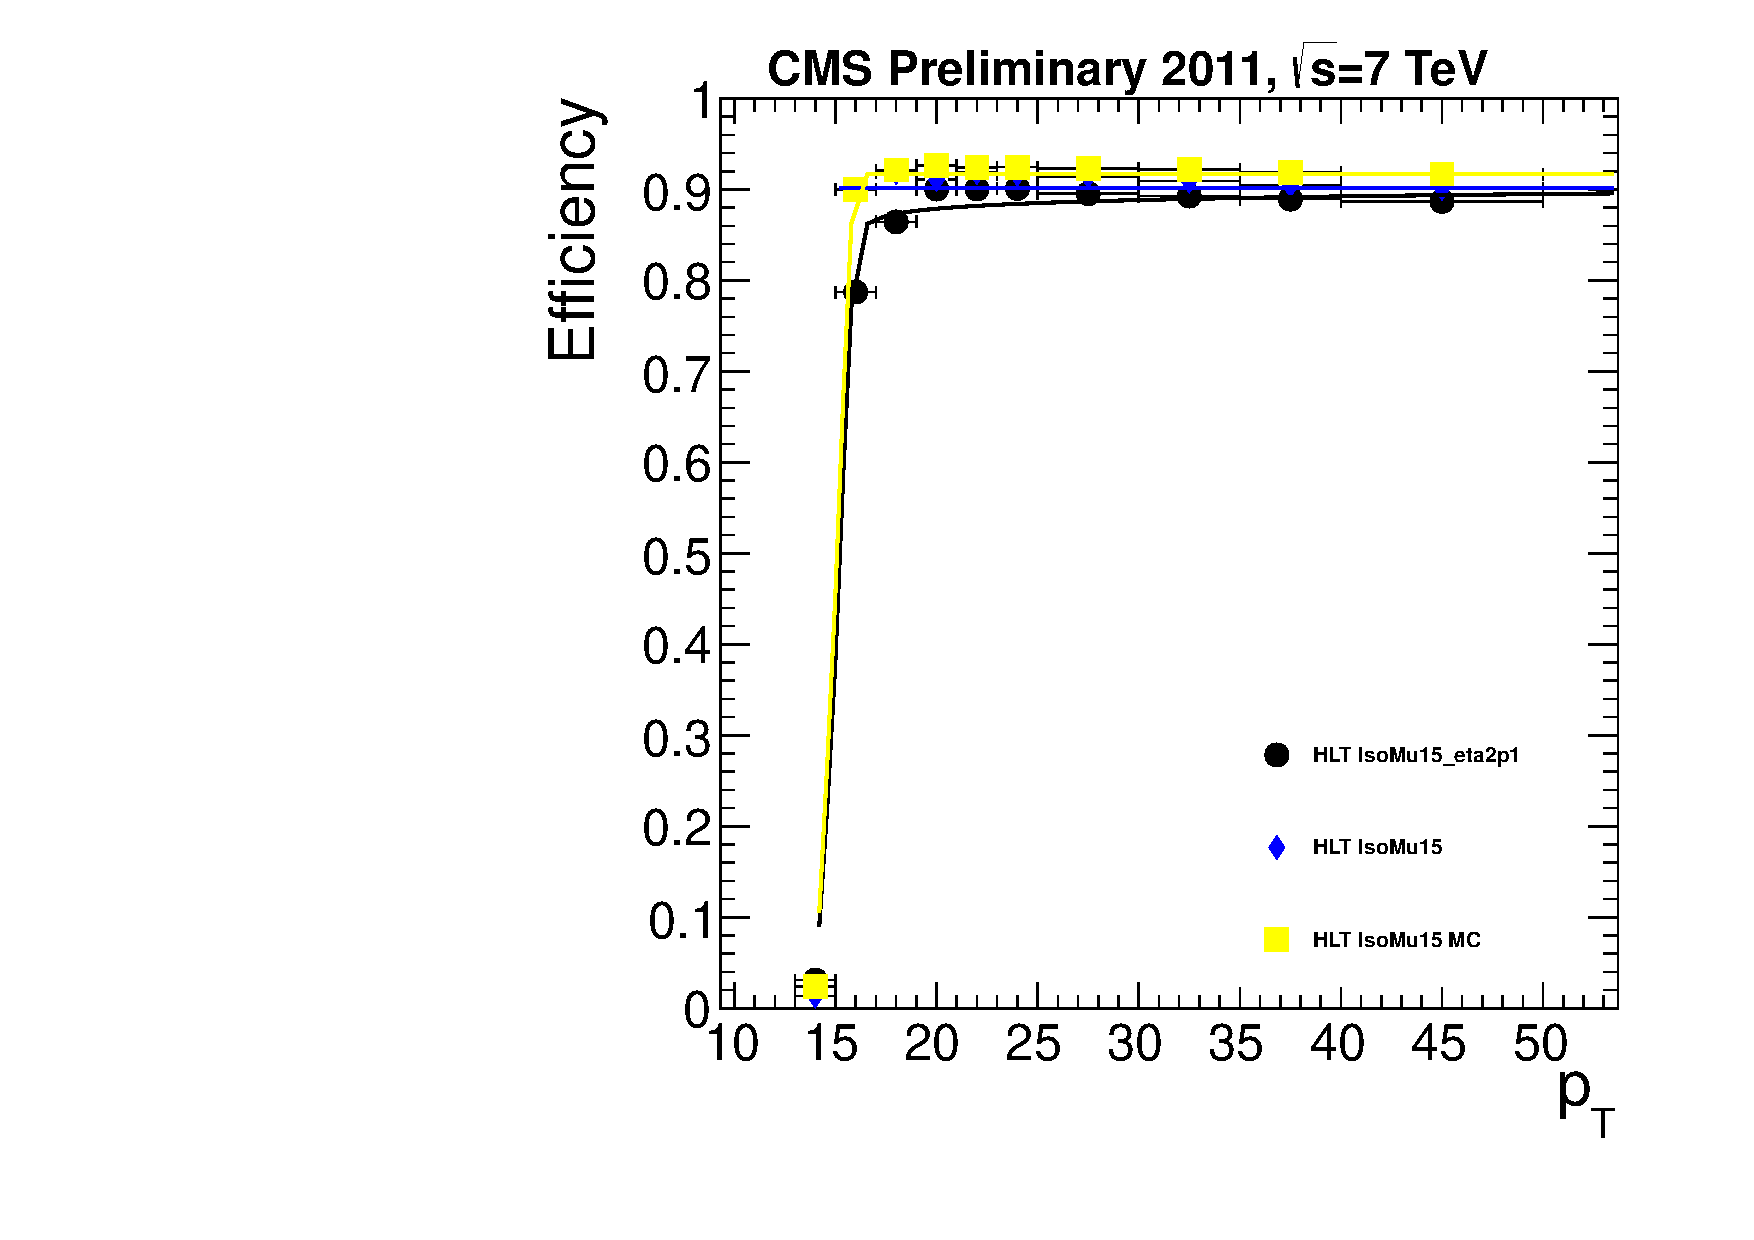
\includegraphics[width=0.9\textwidth]{plots/MuonLegEffB.pdf}
\end{minipage}
\begin{minipage}[b]{0.45\linewidth}
\centering
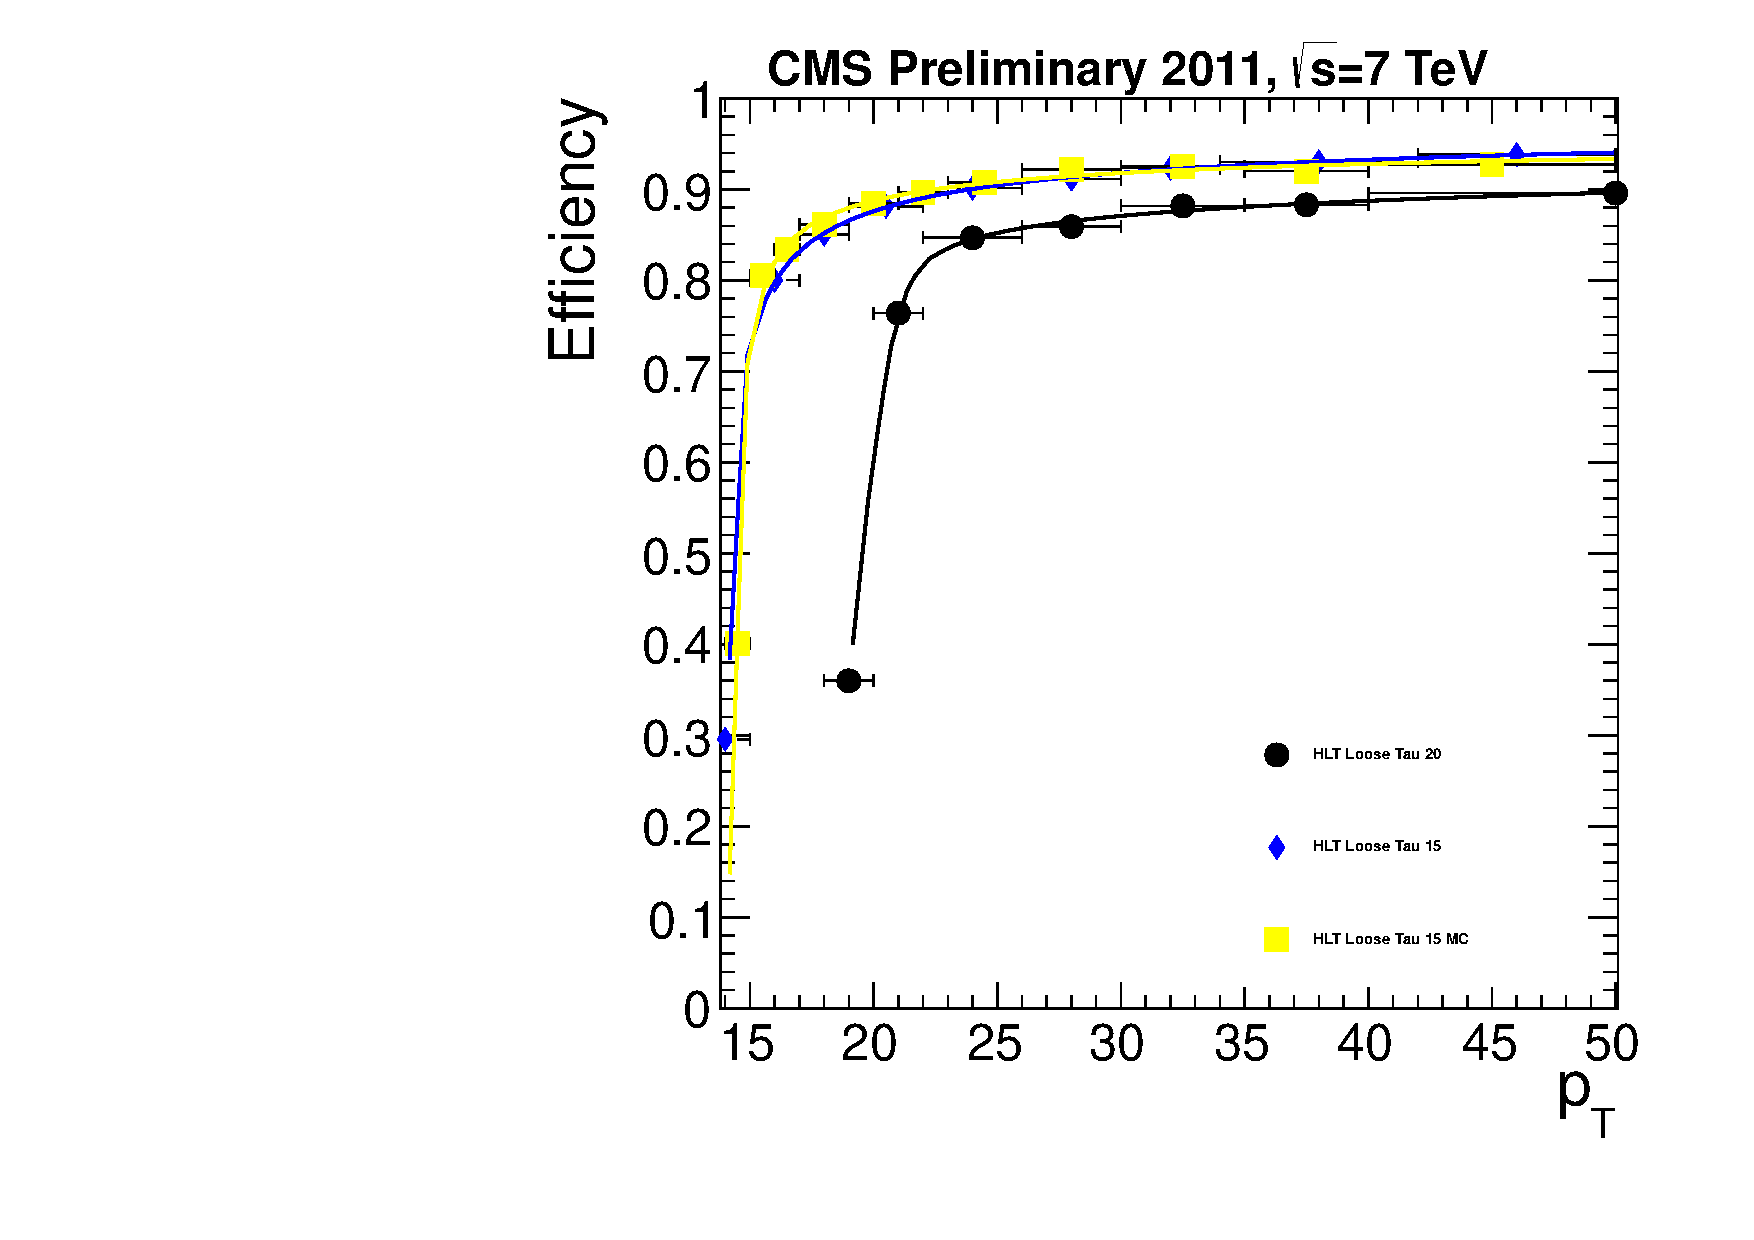
\includegraphics[width=0.9\textwidth]{plots/TauLegEffMuTauB.pdf}
\end{minipage}

\begin{minipage}[b]{0.45\linewidth}
\centering
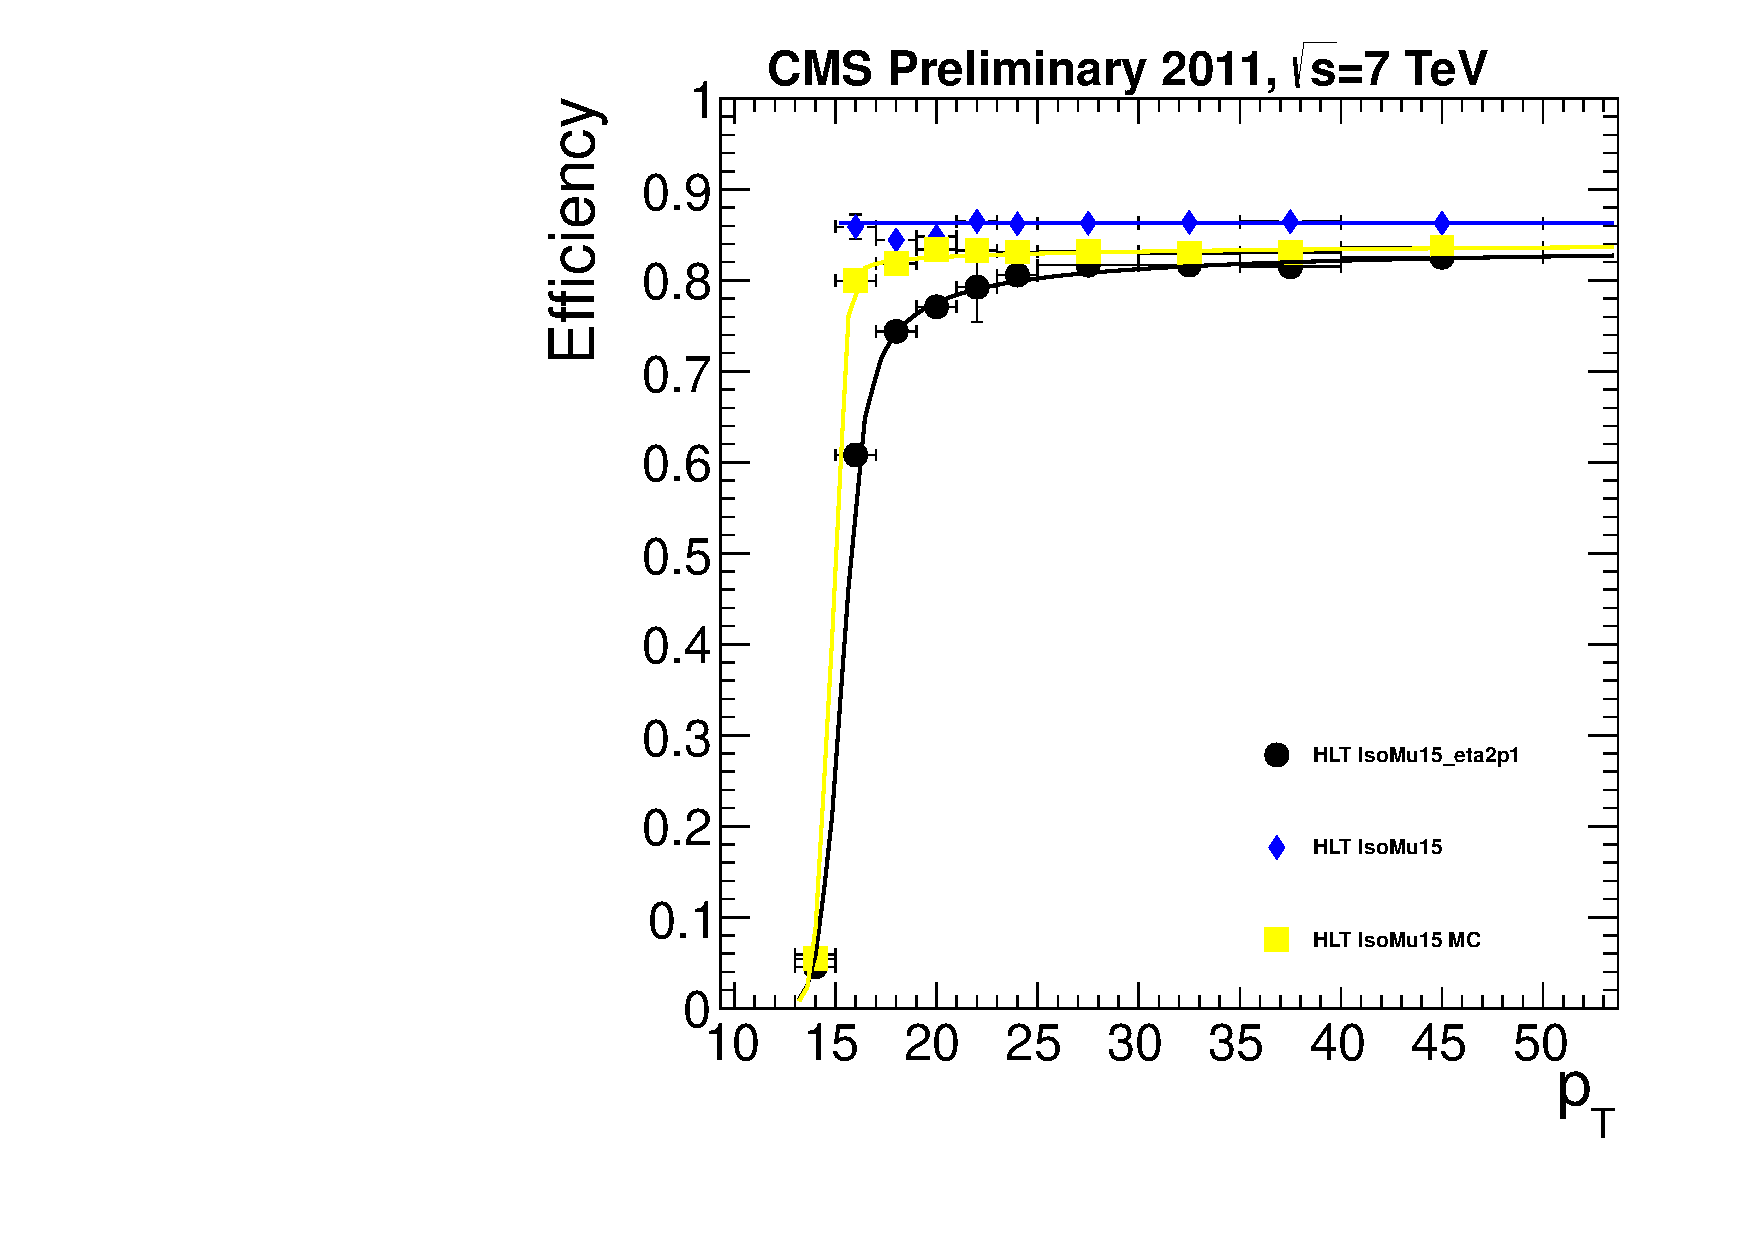
\includegraphics[width=0.9\textwidth]{plots/MuonLegEffE.pdf}
\end{minipage}
\begin{minipage}[b]{0.45\linewidth}
\centering
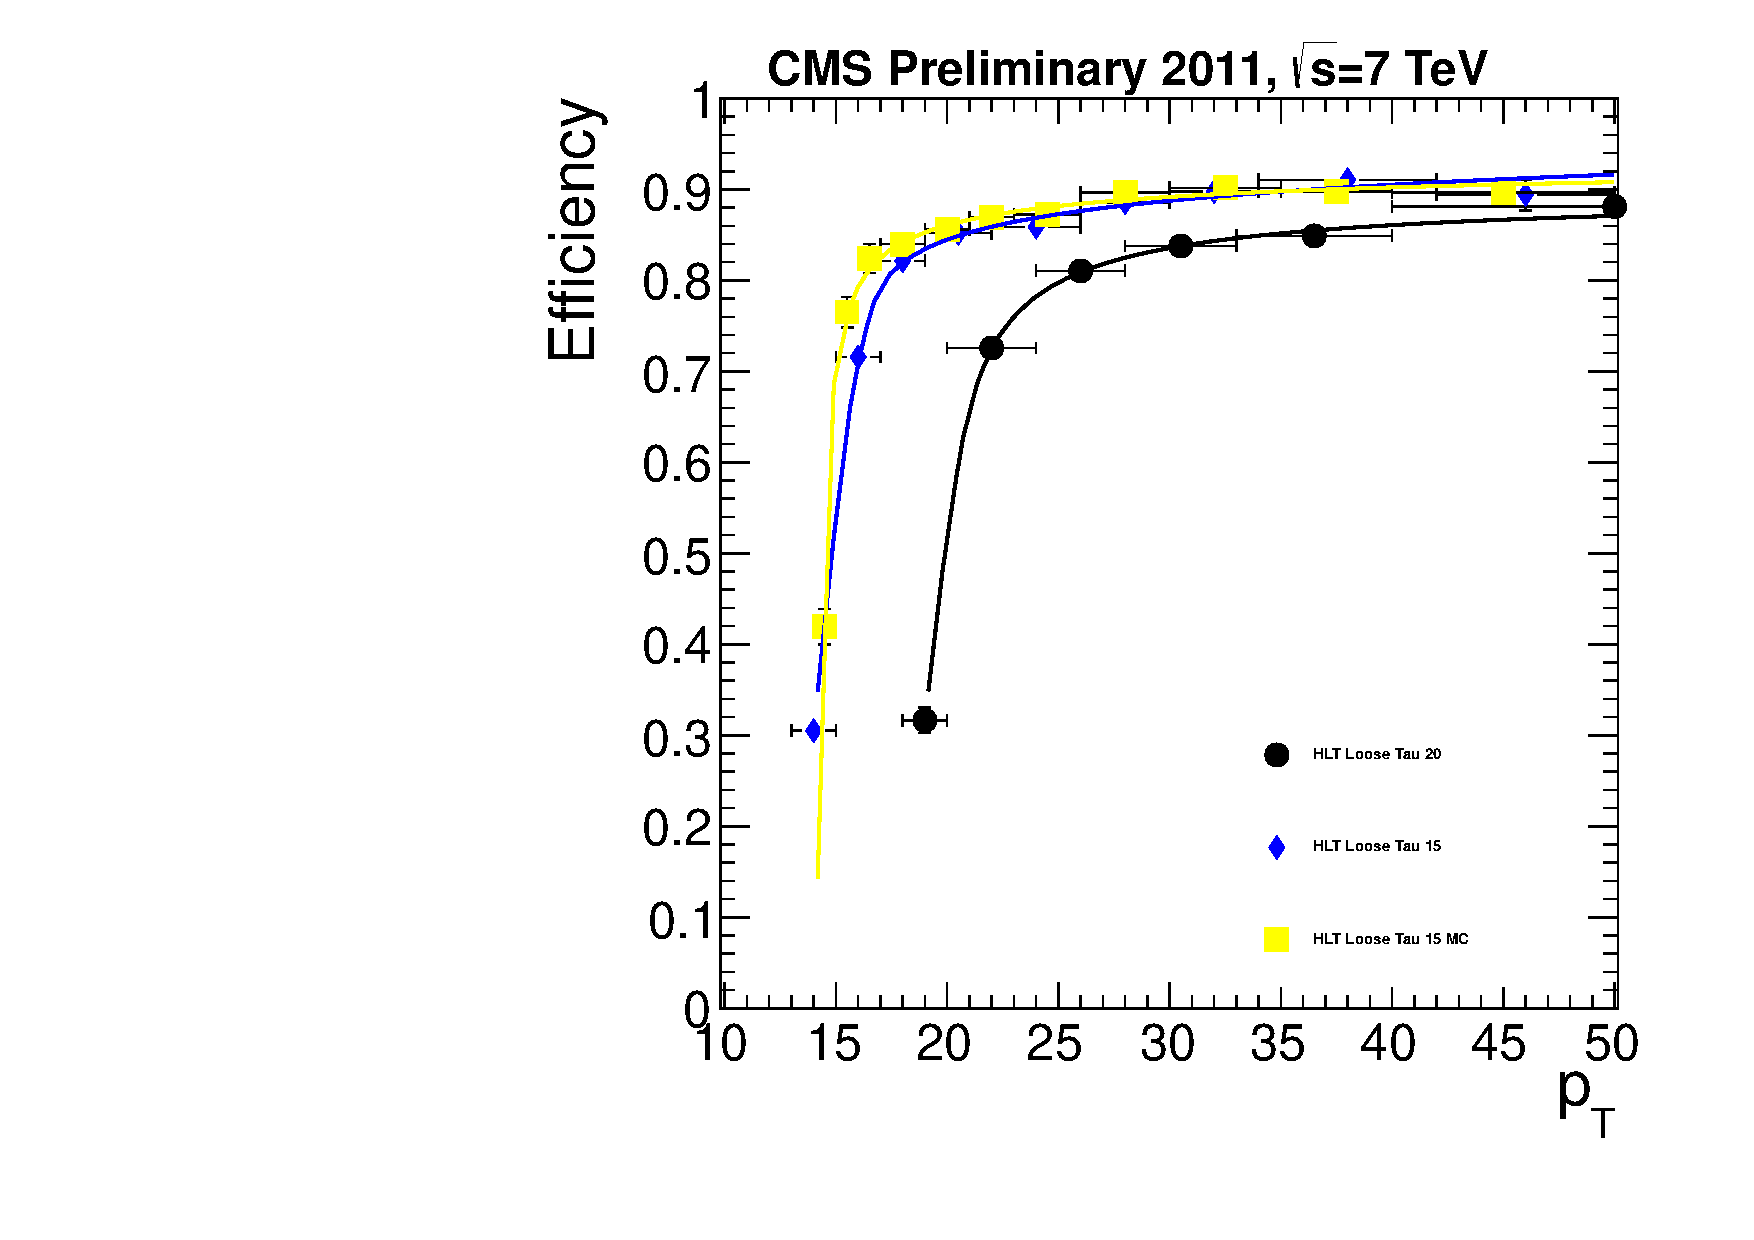
\includegraphics[width=0.9\textwidth]{plots/TauLegEffMuTauE.pdf}
\end{minipage}
\caption{Trigger effeciencies as a function of muon (left) and tau (right) momentum for the barrel (top) and endcap (bottom) regions of the detector.}
\label{fig:turnoncurve}
\end{figure}

A similar procedure is followed to map the efficiency of the tau leg, first selecting a muon that passes the single muon trigger. 
However rather than choosing a probe muon, a probe tau is chosen by making a more loosely selected tau than that described in Section \ref{sec:tauselection}.
The efficiency is again found by fitting an error function to the measured efficiency as a function of the offline reconstructed tau $p_{T}$ and can be seen in the right hand portion of Figure \ref{fig:turnoncurve}, again with the barrel region on top and the endcap region below.

The simulation is then corrected by taking the ratio of the efficiency as measured in simulation to the efficiency as measured in the data.
The final correction is taken as a sum weighted by the luminosity of each trigger used in the data as seen in Table \ref{tab:triggerpaths}.

\subsection{Lepton Selection Corrections}
\label{subsec:leptoncorrections}
The selection efficiencies for muons are calculated with the use of $Z\rightarrow \mu\mu$ events.
A tag and probe method is used in which a tag muon is required to pass all selections listed in Section \ref{sec:muonselection} and match a single muon trigger level object.
The probe muon is then required to satisfy both $p_{T} > 5$ GeV  and $-2.1 < \eta < 2.1$.
The tag and probe muon pairs are then considered if they have opposite charge and an invariant mass within a window around the $Z$ mass: $60 < m_{\mu\mu} < 120$ GeV.
Once tag/probe pairs have been selected, the probe muon is tested to pass the full selection ($N_{pass}$ or $N_{fail}$).
The efficiency is calculated in bins of $p_{T}$, as 
\begin{equation}
\epsilon = {N_{pass}\over N_{pass} + N_{fail}},
\end{equation}
and are summarized in Table \ref{tab:corrections}

\begin{table}[htpb]
\begin{center}
\caption{DATA-DRIVEN CORRECTIONS TO MUON SELECTION EFFICIENCY}
\label{tab:corrections}
\begin{tabular}{lcc}
\hline
$p_{T}$ range & barrel & endcap \\
\hline
%$10<p_{T}<15$ & $0.92\pm0.01$ & $0.98\pm0.01$ \\
$17<p_{T}<20$ & $0.948\pm0.005$ & $0.962\pm0.008$ \\
$30<p_{T}$ & $0.9933\pm0.0003$ & $0.9982\pm0.0004$ \\
\hline
\end{tabular}
\end{center}
\end{table}



\subsection{Pile-up Event Reweighting}
As the luminosity increased throughout the 2011 data taking so too did the number of proton-proton interactions per bunch-crossing.
The effect of an increase in the number of interactions is an increase in pile-up interactions, or multiple events being read out by the detector at the same time.
The number of pile-up interactions affect the analysis in a number of ways, for example lowering various selection efficiencies.
Thus it is important that the simulation be corrected when comparisons to the data are performed.
The interaction multiplicity distributions for simulation and for the collected data are shown in Figure \ref{fig:interactionmultiplicity}.
The interaction multiplicity distributions are first normalized in order to produce the reweighting correction.
The correction is derived as a function of interaction multiplicity by taking the ratio of the simulation to the data multiplicity.
An event weight is then assigned to each simulated event based on the interaction multiplicity of the simulated event.%\cite{PILEUP}.
Assigning an event weight to each simulated event ensures that the interaction multiplicity in simulation will match the distribution as measured in data.
This will remove any bias induced in the simulated mass distribution due to incorrect modelling.

\begin{figure}[ht]
  \begin{minipage}[b]{0.5\linewidth}
\centering
  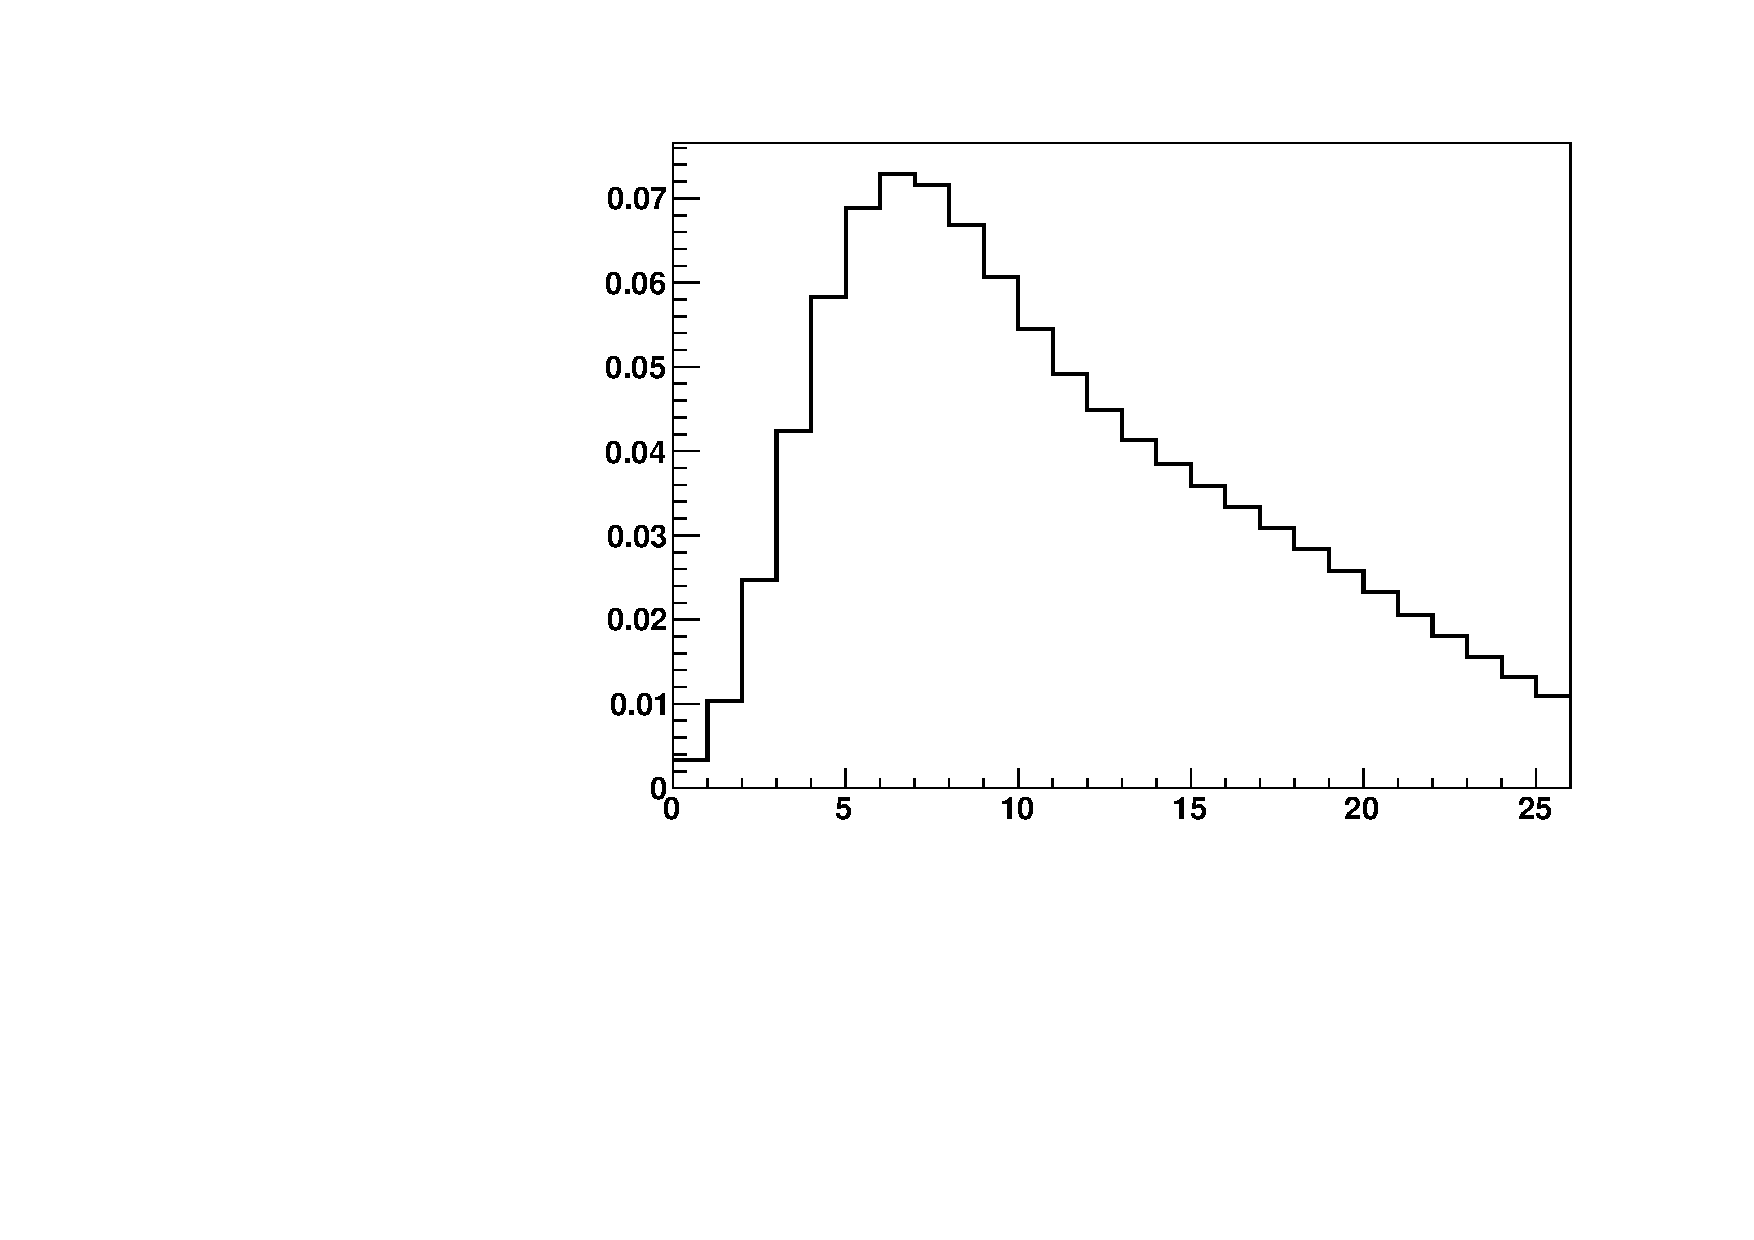
\includegraphics[scale=0.35]{plots/mc_pileup.pdf}
\end{minipage}
\hspace{0.5cm}
\begin{minipage}[b]{0.5\linewidth}
\centering
  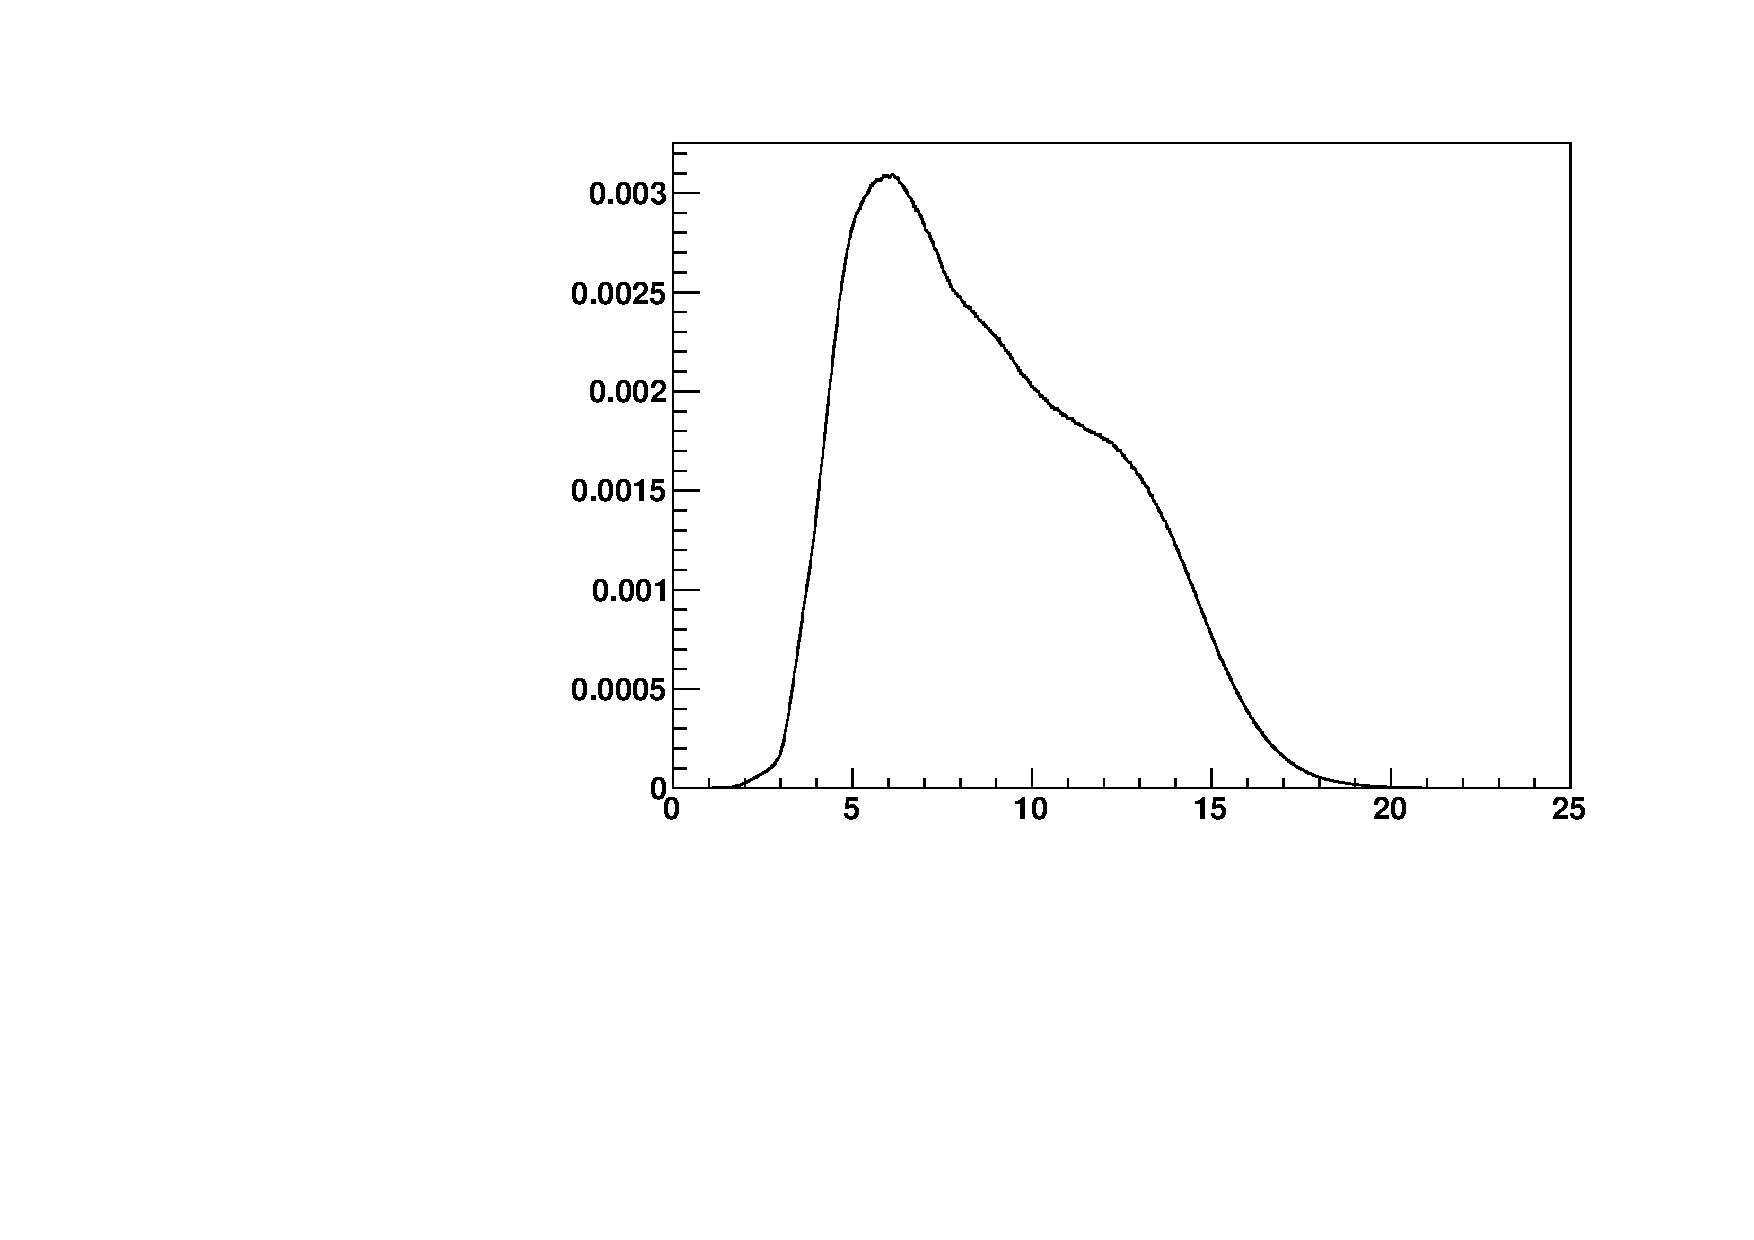
\includegraphics[scale=0.35]{plots/data_pileup.pdf}
\end{minipage}
\caption{Pile-up interaction multiplicity for simulation (left) and the data (right).}
\label{fig:interactionmultiplicity}
\end{figure}


\section{Systematic Uncertainties}
\label{sec:systematics}
\subsection{Normalization Uncertainties}
Each of the efficiency correction factors calculated in Sections \ref{subsec:triggercorrections} and \ref{subsec:leptoncorrections} translates directly into an uncertainty on the final event yield.
This uncertainty is applied as an overall normalization uncertainty determined from the uncertainties in the given measurements.
The combined uncertainty on corrections applied in relation to tau leptons is estimated to be $6.0\%$, and $2.0\%$ for corrections in relation to muons.

The jet energy scale and uncertainty is measured by means of jet balancing in di-jet and $Z/\gamma$+jet events\cite{JETENERGYSCALE}.
An uncertainty of $2.0\% - 5.0\%$ is taken for the true jet energy scale as a function of $p_{T}$ and $\eta$.
The uncertainty on the scale of the jet energy scale is applied as an uncertainty on the yield after being extrapolated to the signal region via a weighted sum given the $p_{T}$ and $\eta$ of the jets in each category.

The uncertainty on the total integrated luminosity will enter the analysis by means of an uncertainty on the normalization of the signal simulation and in any background simulations that have been scaled by the luminosity, e.g. $Z\rightarrow\tau\tau$.
An uncertainty on the luminosity measurement of $4.5\%$ is applied as an uncertainty on the normalization of all signal samples and background samples for which the normalization is taken from simulation\cite{LUMI}. The uncertainty on the $Z \rightarrow \tau\tau$ normalization is taken as $2.5\%$ from the inclusive cross section measurement made by the CMS Collaboration\cite{Z_TAUTAU_CROSS_SECTION}. 
However, rather than taking the uncertainty on the integrated luminosity as an uncorrelated uncertainty, a reduced uncertainty of $2.0\%$ is taken as the uncorrelated portion of the uncertainty
The combined normalization uncertainty on the $Z\rightarrow\tau\tau$ background is then $3.2\%$. 

The normalization of the backgrounds arising from $Z \rightarrow \mu\tau_{jet}$ events results in an uncertainty between $20\% - 25\%$ derived by the uncertainty in extrapolating from the control region into the signal region.
Likewise the uncertainty on the background related to the process $Z\rightarrow\mu\tau_{\mu}$ is between $0.01\% - 0.04\%$, which is driven down by the large number of $Z\rightarrow\mu\mu$ events in the control region for this process.
For the categories \emph{Zero/One Jet}, \emph{B-Tagged} and \emph{Non B-Tagged}, the extrapolation method for estimating the $t\overline{t}$ background produces an uncertainty of $4.1\%$, $2.5\%$, and $4.1\%$ respectively, while for the \emph{Boost} and \emph{VBF} the normalization is taken from the CMS cross section measurement similar to the procedure followed for the $Z\rightarrow\tau\tau$ background and is estimated to be $7.5\%$.
In a similar fashion the uncertainty on the normalization of the $W$ background contribution is obtained from the uncertainty in extrapolating from the control region into the signal region yielding a value of $7\%$ across all categories. 

\subsection{Shape Uncertainties}
In addition to pure normalization uncertainties related to the rate of each process, there are additional uncertainties that will modify the shape of the $m_{\tau\tau}$ distribution for a given process as taken from the simulation.
The variables that contribute to the uncertainty on the distribution are the $p_{T}$ of the muon, the energy of the tau, and the $\met$.
The source of these uncertainties is ultimately due to inaccuracies in the simulation. 
Rather than correct these inaccuracies, however, they are taken into account via a shape uncertainty.
The shape uncertainty is accounted for by varying the variable of interest up and down by one standard deviation, producing the scenarios in which the variable is shifted up and down.

\subsection{Theory Uncertainties}
In addition to the previously discussed uncertainties additional uncertainties related to theoretical calculations must be taken into account.
The first theoretical uncertainty to be considered is the uncertainty of the parton-distribution functions (PDFs) that describe the distribution of momentum shared among the constituents of the colliding protons.
This uncertainty is taken to be $3.0\%$ and is derived from \cite{PDFUNCERTAINTY}.

In the standard model search the uncertainty on the dependence of the signal acceptance on the Higgs production mechanism and branching ratio are taken directly into account in the cross section measurement.
This includes the uncertainty on the gluon-gluon fusion and vector-boson fusion production mechanisms ($gg \rightarrow H$ and $qq \rightarrow Hqq$ respectively)\cite{HIGGS_PRODUCTION}.
In the MSSM search the production mechanism uncertainty is used when translating the cross section measurement to a search in $M_{A}-tan\beta$ space.

